\chapter{Обзор и анализ источников}
\section{Модели легких}
Легкие – жизненно важные органы, ответственные за обмен кислорода и углекислого газа в организме человека и выполняющие дыхательную функцию. Когда легкие расширяются, свежий воздух поступает в их газообменные отделы по системе ветвящихся трубок. Вначале он проходит через трахею, затем через два главных бронха и далее через все более мелкие ветви бронхиального дерева. Вплоть до 16-го ветвления, за которым следуют конечные бронхиолы, единственная функция дыхательных путей состоит в проведении воздуха. После 17-19-го делений образуются дыхательные бронхиолы, в стенках которых уже имеются отдельные альвеолы. После 20-го деления начинаются альвеолярные ходы, плотно окруженные альвеолами. Эта зона легких, выполняющая главным образом функцию газообмена, называется дыхательной зоной. Размер ветвей также очень сильно различается: ~1.5 сантиметра составляет радиус на уровне трахеи и порядка нескольких десятков микрометров на уровне альвеолярных ходов \cite{schmidt}.

Механика дыхания уже достаточно долго находится в сфере интересов многих исследователей. Основные ее положения были сформулированы еще в середине XIX века. Через 70 лет Роэром был разработан обобщающий количественный подход, который затем был развит и доведен до экспериментальных наблюдений его учениками. Тем не менее, широкое экспериментальное изучение вопроса было начато лишь в начале XX века.

Наиболее простой и универсальный подход к моделированию, основные его положения были сформулированы в середине XX века, связан с однокомпонентным представлением легкого.
Легкое представляется в виде резервуара переменного объема, для описание которого используются осредненные механические параметры, такие как сопротивление, эластичность, инерционность \cite{Dyachenko1986}.
\begin{equation}
    C\frac{dP_{in}}{dt}+Q_{out}-Q_{in}=0
\end{equation}
\begin{equation}
    I\frac{dQ_{out}}{dt}+RQ_{out}+P_{out}-P_{in}=0
\end{equation}
где $R$ ~-- сопротивление, $C$ ~-- эластичность,  $I$ ~-- инерционность, $P_{in}$ ~-- давление на входе в дыхательные пути, $P_{out}$ ~-- давление на выходе из дыхательных путей, $Q_{in}$ ~-- поток, направленный в дыхательные пути, $P_{out}$ ~-- поток, направленный из дыхательных путей.   

Для учета структуры трахейно-бронхиального дерева используются модели, связанные с применением электромеханических аналогий. Для описания легких на основе электромеханических аналогий используются следующие параметры:

a) Сопротивление дыхательных путей, связанное с диссипативными вязкостными эффектами.
\begin{equation}
    \triangle P=R \cdot Q
\end{equation}

В случае течения Пуазейля:
\begin{equation}
R_{p}=\frac{8\mu L}{\pi r_{aw}^{4}}
\end{equation}
где $Q_{in}$ ~-- длина дыхательных путей, $r_{aw}$ ~-- радиус дыхательных путей, $\mu$ ~-- динамическая вязкость воздуха.
Данная формула не всегда корректна для верхних дыхательных путей, в которых течение может быть турбулентным. Для учета нелинейных эффектов используется сопротивление в виде \cite{Pedley1970}:
\begin{equation}
R=\gamma \left( Re \frac{D}{L}\right)^{0.5} R_{p}
\end{equation}
где $D$ ~-- диаметр дыхательных путей, $Re$ ~-- число Рейнольдса, $\gamma = 0.327$. Число Рейнольдса определяется из выражения:
\begin{equation}
Re=\frac{4\rho \mid Q\mid}{\mu \pi D}
\end{equation}
где $\rho$ ~-- плотность воздуха.
Для исклучения возникновения сингулярности при нулевом потоке выражение может быть преобразовано к виду:
\begin{equation}
R=
\begin{cases}
\gamma \left( Re \frac{D}{L}\right)^{0.5} R_{p}; & R \ge R_{p}\\
R_{p}; & R < R_{p}
\end{cases}
\end{equation}
Для дифференцирования в $R=R_{p}$ используется сигма функция:
\begin{equation}
R=\gamma \left( Re \frac{D}{L}\right)^{0.5}\zeta(Re)+\left(1-\zeta(Re)\right)R_{p} 
\end{equation}
где
\begin{equation}
\zeta(Re) = \frac{1}{1+e^{-k\left(Re-R_{p}\right)}}
\end{equation}
Другой подход для расчета сопротивления состоит в использовании эмпирических соотношений на основе уравнения Роэра \cite{Reynolds1979,Lambert1982,Ertbruggen2005}:
\begin{equation}
 \triangle P=K_{1}Q+K_{2}Q^{2}
\end{equation}

б) Эластичность дыхательных путей:
\begin{equation}
\frac{d\triangle P}{dt}=\frac{Q}{C}
\end{equation}
\begin{equation}
C=\frac{2Lr_{aw}^{3}}{E_{aw}t_{aw}}
\end{equation}
где $E_{aw}$ ~-- эластичность стенки, $t_{aw}$ ~-- толщина стенки, $r_{aw}$ ~-- радиус.

в) Инерционность дыхательных путей:
\begin{equation}
\triangle P=I\frac{dQ}{dt}
\end{equation}
\begin{equation}
I=\frac{L\rho}{\pi r_{aw}^{2}}
\end{equation}
Влияние данного члена становится значительным при большой чистоте вентиляции.

Таким образом на основе электромеханических аналогий существует четыре типа моделей: R, RC, RLC, вязко-эластичная-RLC.
\begin{figure}[!ht]
	\centering
	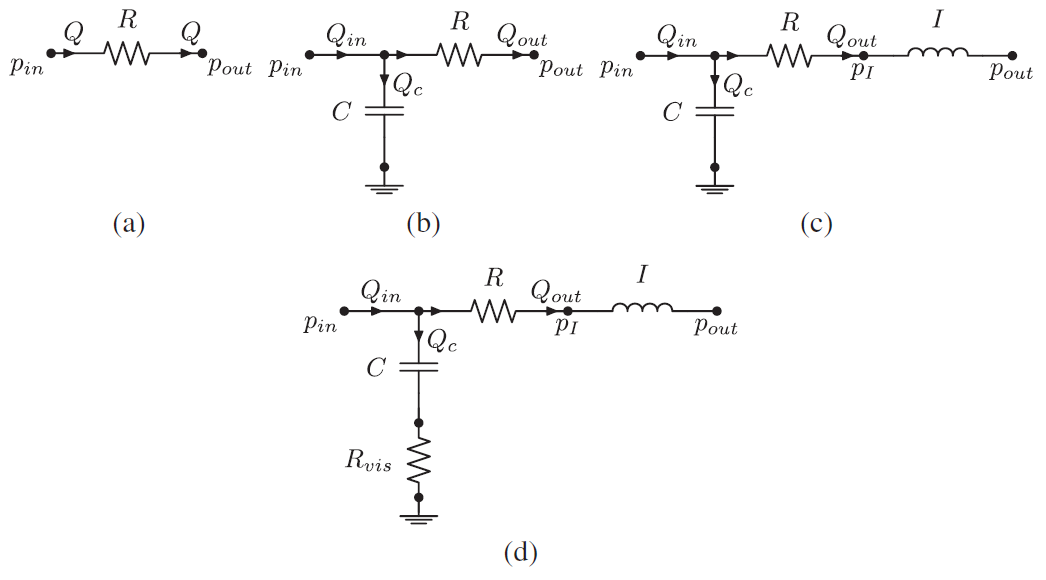
\includegraphics[scale=0.55]{review1}
	\caption{a) R-модель, b) RC - модель, c) RLC - модель, d) вязко-эластичная-RLC модель } 
\end{figure}
Преимущество данного подхода – использование хорошо изученной теории электрических цепей, а также возможность применения в комплексных моделях, которые включают в себя многочисленные подсистемы, как элемент, описывающий работу системы дыхания.   Недостаток состоит в том, что повышение степени детализации приводит к значительному усложнению описываемых уравнений. Также данные уравнение при любых модификациях сети следует выводить заново \cite{Bates2009}.    

Параметры моделей на основе электромеханических аналогий, а также других 1D моделей \cite{Suki1993, Lutchen1996,Gillis1999,Nucci2002} могут быть аккуратно подобраны для достижения хорошего соответствия с экспериментальными данными. Однако точный расчет для всех областей трахейно-бронхиального дерева только с использованием 1D моделей не может быть выполнен. Данное ограничение связано с разрешающей способностью изображений компьютерной томографии(CT). Вместо CT-данных может быть использована модельная структура трахейно-бронхиального дерева, например \cite{Horsfield1971,Weibel1963}, с помощью которой можно выполнить расчет во всех областях легких. Недостаток такого метода очевиден-он не является пациенто-ориентированным. Более универсальным является гибридный подход, в котором крупные пути получаются на основе CT-изображений, а мелкие структуры генерируются с помощью специальных алгоритмов заполнения данных \cite{Tawhai2000,Tawhai2010,Tawhai2006,Lin2009}. 

Для моделирования динамики мелкой альвеолярной структуры, помимо описанных выше 0-D моделей, популярной является четырехэлементная модель Максвелла \cite{Bates2009,Denny2000}:
\begin{equation}
B\frac{d^{2}P(t)}{dt^{2}}+E_{2}\frac{dP(t)}{dt}=B_{a}B\frac{d^{2}Q_{i}}{dt^{2}}+\left(E_{1}B+E_{2}B+E_{2}B_{a}\right)\frac{dQ_{i}(t)}{dt}+E_{1}E_{2}Q_{i}(t)
\end{equation}
\begin{equation}
P=P_{a}-P_{pl}
\end{equation}
\begin{equation}
P(w)=\left(E_{dyn}+jwR_{dyn}\right)\triangle V_{i}(w)
\end{equation}
\begin{equation}
\triangle V_{i}=V_{i}-V_{i}^{0}
\end{equation}
\begin{equation}
E_{dyn}=\frac{w^{2}B^{2}(E_{1}+E_{2})+E_{1}E_{2}^{2}}{E_{2}^{2}+w^{2}B^{2}}
\end{equation}
\begin{equation}
R_{dyn}=\frac{E^{2}_{2}(B+B_{a})+w^{2}B_{a}B^{2}}{E_{2}^{2}+w^{2}B^{2}}
\end{equation}
\begin{figure}[!ht]
	\centering
	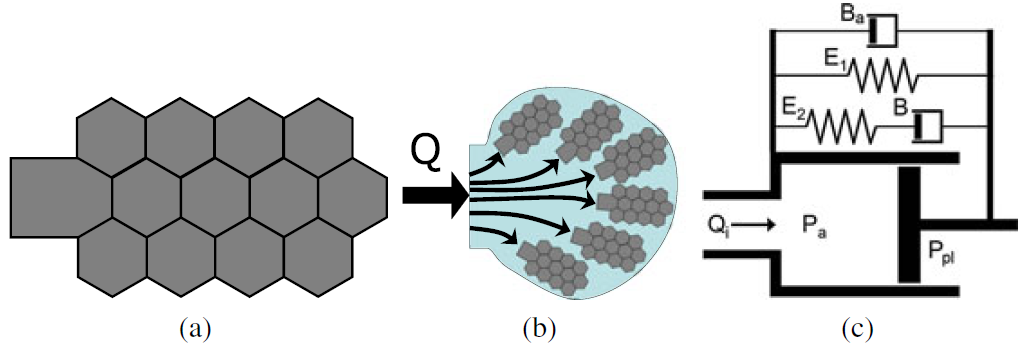
\includegraphics[scale=0.55]{review2}
	\caption{Четырехэлементная модель Максвелла } 
\end{figure}
Для более детального описания динамики потоков воздуха внутри легких (актуально, например, в задачах расчета эффективности ингаляции различных препаратов) используется классические трехмерные подходы вычислительной гидродинамики (CFD) с использованием уравнений Навье-Стокса либо метода частиц, часто в сочетании с моделями турбулентности. При этом расчетной областью является трехмерная геометрическая модель трахейно-бронхиального дерева (иногда с добавлением геометрии носоглотки), полученная либо из аналитического выражения на основе статистики по большому количеству людей, либо персонифицированная геометрия на основе обработки CT-данных конкретного человека. Несомненным преимуществом такого подхода является возможность исследования сложных неоднородных потоков внутри легких, а также возможность учета их индивидуальных анатомических особенностей строения. К недостаткам метода относятся сложность построение расчетной сетки (размеры трубок могут отличаться на несколько порядков, и поэтому сложно качественно рассчитывать течение одновременно в больших и малых трубках), большие требования к вычислительным ресурсам \cite{Zhang2002,Liu2002,Green2004,Zhang2004,Lin2007,LDe2008,Wall2008}. 
\begin{figure}[!ht]
	\centering
	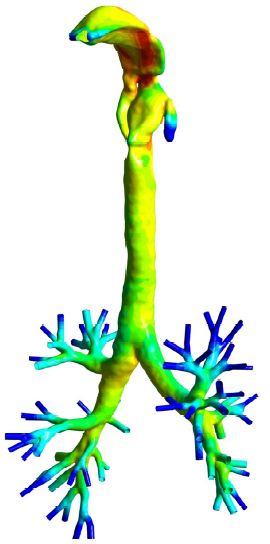
\includegraphics[scale=0.55]{review4}
	\caption{Модель легких на основе CFD подхода } 
\end{figure}
Для использования преимуществ одномерных и трехмерных моделей делаются попытки по их объединению, когда для верхних дыхательных путей используется 3D уравнения Навье-Стокса и CT-геометрия, а мелкие структуры описываются на основе осредненных 0-1D моделей \cite{Lin2009,Ma2006,Comerford2010,Yoshihara2013,Yin2010}. В данном алгоритме расчета возникают проблемы с корректной постановкой граничных условий. Подходы к решению данной проблемы описаны в \cite{Lin2009,Ma2006,Comerford2010,Yin2010,Quarteroni2003,Formaggia2000,Fernandez2005}.
\begin{figure}[!ht]
	\centering
	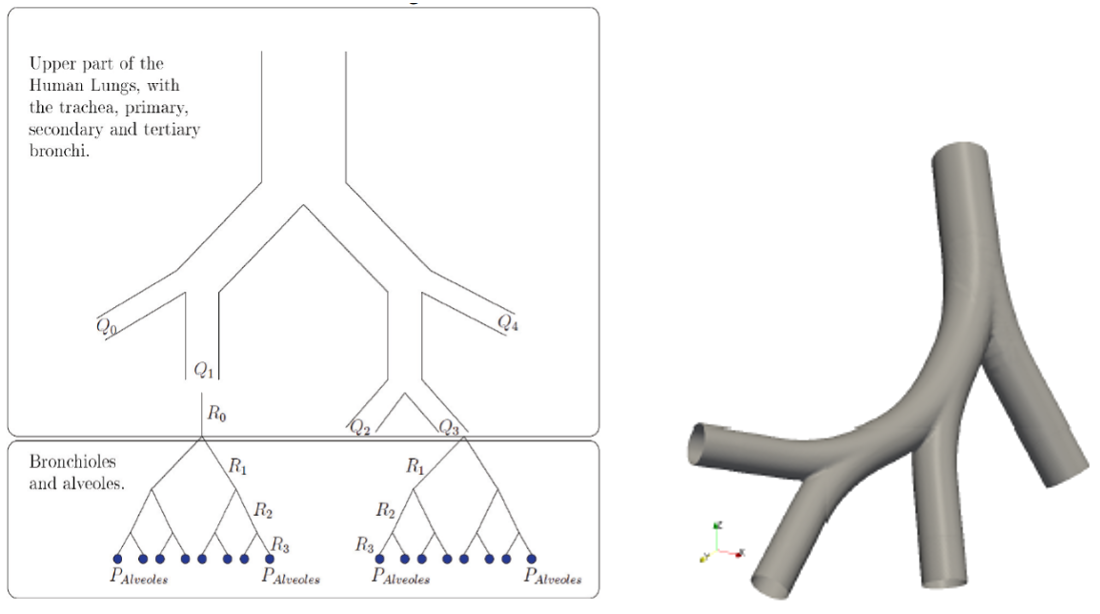
\includegraphics[scale=0.45]{review3}
	\caption{Гибридная 3D-1D модель } 
\end{figure}
Для еще более точного расчета 3D-потока, в ряде работ учитывается деформация стенок трахейно-бронхиальных трубок и используется fluid-structure interaction(FSI) подход. Также альвеолярные объемы представляют в виде шариков, деформацию которых под действием потоков воздуха рассчитывают на основе уравнений смещения в упругих, эластичных материалах.  В этом случае требования к вычислительным ресурсам еще больше возрастают.

\textit{Модели дыхательной системы можно классифицировать по размерности пространства. Наиболее точным при расчете верхних дыхательных путей являются 3D модели, в которых решаются уравнения Навье-Стокса и используются модели турбулентности внутри CT~---геометрии легких. К недостаткам данного подхода можно отнести большие затраты вычислительных ресурсов. Для более мелких путей эффективным является применение 1D и 0D подходов, в которых решаются усредненные уравнения для трубок или объемов. Наиболее перспективными сейчас являются гибридные многомасштабные модели. }

\section{Модели кровеносной системы}

Для кровеносной системы также применяется метод электромеханической аналогии. При правильном подборе параметров электрической цепи модель
дает достаточно точное описание волновых процессов кровотока \cite{Hassani2006,Mynard2012}. Недостатком
является неоднозначность соответствия между системой кровеносных сосудов
и электрической цепью, а также высокая сложность уравнений при увеличении
детализации системы. Модели данного класса могут использоваться как промежуточные для стыковки других моделей разных масштабов.   
\begin{figure}[!ht]
	\centering
	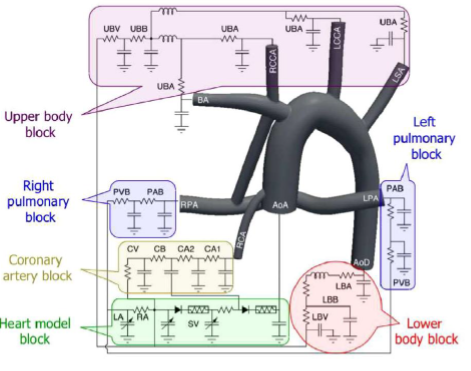
\includegraphics[scale=0.75]{review5}
	\caption{Детальная 3D-модель аорты, электромеханическая модель оставшейся подсистемы} 
\end{figure}
Другой распространенный подход связан с разделением кровеносной системы на отдельные связанные подсистемы (компартменты), соответствующие крупным участкам. При этом для каждого отдельного компартмента может дополнительно решаться своя система уравнений, например связанная с биохимией \cite{Blanco2016}.  

Для более детального расчета пульсирующих потоков в кровеносном русле используются одномерные модели на основе уравнений механики сплошных сред для вязкой несжимаемой жидкости на графе тонких эластичных, деформируемых трубок.  Обычно используются допущения, что отношение диаметра сосуда к его длине относительно невелико, а поле скорости демонстрирует профиль Пуазейля на каждом поперечном сечении. Гемодинамическая модель замкнутой (глобальной) циркуляции состоит из уравнений одномерной кровотока в отдельных сосудах, связанных граничными условиями в точках соединения сосудов и сердца \cite{Simakov2009,Kholodov2006,Vassilevski2011,Bessonov2016,Sherwin2003}.

Основным преимуществом одномерной модели является возможность целиком рассчитывать замкнутую кровеносную систему, состоящую из большого числа сосудов, с использованием незначительного количества компьютерных ресурсов. Недостаток – грубые результаты расчетов. Данную проблему позволяю преодолевать двумерные и трехмерные модели, которые предоставляют возможность достаточно точно рассчитать движение крови в рамках отдельного сосуда, сопряжения сосудов или отдельного участка кровеносной системы. Но в этом случае возникают те же сложности, что и при моделировании дыхательной системы таким способом. 

Для детального описания пространственного профиля течения используются двух- и трехмерные уравнения Навье–Стокса. Это дает возможность хорошо изучить многие эффекты, наблюдаемые при движении крови в рамках одного или нескольких соединенных между собой сосудов, например, завихрения потока крови в области стыковки сосудов \cite{Xiao2013,Yakhot2005}.

Особое внимание уделяется не только рассмотрению уравнений течения крови, но и моделированию стенок сосудов, так как сложность заключается в рассмотрении объединенной модели «стенка сосуда – поток крови». Более подробный обзор этой проблемы может быть найден, например, в \cite{Vito2003,Humphrey2003}. В том числе, делаются попытки построения определяющих соотношений, на основе внутренней микроструктуре стенок сосудов \cite{Chen2013}. Современные методики решения данной проблемы также основываются на FSI подходе – совместном решении уравнений Навье-Стокса для крови и уравнений механики твердого деформируемого тела для эластичных сосудов. Развитие и распространение современных высокопроизводительных кластеров дает возможность более активно использовать данный высокоточный подход \cite{Crosetto2011,Barker2010}.

Для моделирования работы сердца на сегодняшний день существует несколько метод. В самом простом случае сердце задается как граничное условие, зависящее от времени (аналогично электромеханическому подходу) \cite{Carlo2003}. В более сложных моделях сердце представляется в виде нескольких резервуаров, соединенных сосудами. Каждый резервуар выбрасывает кровь в соседний при выполнении определенных условиях (наполнение до критического объема или по прошествии определенного промежутка времени) \cite{kholodov2001}. 

\textit{Подходы к моделированию сердечно-сосудистой системы во многом схожи с теми, что используются при моделировании дыхательной системы и имеют аналогичные преимущества и недостатки. Различия связаны с наличием сердечной мышцы, более сложным, нелинейным поведением стенок сосудов.}


\section{Модели связывания кислорода и углекислого газа в крови}
Первым модель, описывающую связывание кислорода гемоглобином опубликовал Хилл \cite{Hill1910}. Он предложил использовать кинетическую реакцию, состоящую из одной стадии, а кривую сатурации описывать уравнением  n-го порядка и зависимостью от двух параметров:
\begin{equation}
S_{O_{2}} = \frac{K_{O_{2}}P_{O_{2}}^{n}}{1+K_{O_{2}}P_{O_{2}}^{n}}
\end{equation}
где $P_{O_{2}}$ ~-- парциальное давление кислорода, $K_{O_{2}}$ ~-- коэффициент Хилла, $n$ ~-- степень Хилла.

Из экспериментальных данных были получены значения $n=2.7$, $K_{O_{2}}=1.39 10^{-4}  mmHg^{-1}$, при этом сатурация варьируется в пределах 20-98\%. 

Айдаром \cite{Adair1925} была предложена более реалистичная модель, описывающая 4х- стадийную модель кинетики. Уравнение сатурации уже включало в себя четыре параметра. Хорошая точность модели позволила применять ее для анализа экспериментальных данных в широком диапазоне парциальных давлений кислорода. 

Винслоу \cite{Winslow1983} описал модель, позволяющею учитывать влияние на сдвиг кривой диссоциации помимо парциального давления кислорода, парциальные давления углекислого газа pH и концентрацию дифосфонооксипропановой кислоты (DPG).   

Кельман \cite{Kelman1966} разработал алгоритм для расчета концентрации углекислого газа в зависимости от уровня pH, температуры крови, сатурации кислорода. Форстер исследовал скорость реакции преобразования углекислого газа и гемоглобина в карбамино-гемоглобин при различных физиологических условиях. 

Хуанг и Геллумс \cite{Huang1994} разработали модель конвективно-диффузионного переноса кислорода и углекислого газа в соответствии с кислотно-щелочным равновесием, а также учли эффекты Бора и Холдена (увеличение парциального давления углекислого газа или pH уменьшает сродство кислорода и гемоглобина, увеличение парциального давления кислорода уменьшает сродство углекислого газа и гемоглобина). 

Для комплексного учета всех основных факторов на сатурацию кислорода и углекислого газа часто используются полуэмпирические модели \cite{Christensen1996,Siggaard1984,Christensen2004}. Наиболее полная модель и строгая модель с точки зрения химической кинетики описана в работах Даша \cite{Dash2010}.  

Если необходимо учесть влияние буферных систем крови на уровень pH, то распространенной является модель \cite{Chiari1994}.

\textit{Взаимодействие кислорода и углекислого газа с кровью является достаточно сложным и включает в себя большое количество реакций. Подробное описание всех процессов значительно усложняет модель. При расчете глобального переноса обычно рассматриваются ключевые для задачи реакции либо используются некоторые эмпирические соотношения.}

\section{Совместные модели дыхательной и кровеносной систем}
Математические модели для совместного моделирования дыхательной и кровеносных систем активно разрабатывались с середины 20го века \cite{GuytonColeman1972,Grodins1967}. С того момента было предложено большое количество работ применительно к различным областям исследования. Например, теория управления \cite{Grodins1967,Gray1946,Reyes2014,Mauro1998,Ursino1994,Batzel2007,Ottesen2004,Chiari1997,Magosso2001}, анализ чувствительности и оценки параметров  \cite{Batzel2010,Fink2008,Kappel2006}, изучение патологий  \cite{Khoo2008} и пациенто-ориентированное моделирование \cite{Ottesen2014,Ellwein2013,Williams2013}. В работе \cite{Ursino2001} описана модель дыхательной и кровеносной системы, включавшая в себя кривые диссоциации кислорода и углекислого газа, а также механизмы регуляции. В данной модели используется достаточно простое представление каждой отдельной подсистемы. Аналогично, в \cite{Batzel2011} рассматривается реакция организма при воздействии гиперкапнии основываясь на модели \cite{Ellwein2013,Olufsen2013}. Некоторые модели описывают влияние легочной механики на гемодинамику \cite{Hardy1982,Lu2001,Hemalatha2010}. Достаточно всеобъемлющая модель описана в \cite{Blanco2016}, которая основывается на усредненной модели подотделов дыхательной и кровеносной систем и включает в себя тканевый метаболизм, диссоциацию кислорода и углекислого газа.

\textit{Совместные модели дыхательной и кровеносной систем обычно используются для описания глобальных процессов в организме. В большинстве случаев применяются усредненные модели. В зависимости от решаемой практической задачи, детализации подвергаются отдельные подсистемы.}

\section{Модели регуляции}
Описании контроля дыхания с использованием теории управления было выполнено в работах Грея \cite{Gray1946} и Дефареса \cite{Defares1964}. Кху и соавторы \cite{Khoo1982} предложили общую модель, учитывающую нелинейность регулятора дыхания. Модель была специально разработана для исследования устойчивости системы, и она способна учитывать несколько видов периодического дыхания, вызванного нестабильностью дыхательного контроля: в нормальном состоянии во время сна и при сильном воздействии на большой высоте, у спящих детей и у пациентов с сердечно-сосудистыми или неврологическими отклонениями. Первая же общая модель была предложена Гродинсом \cite{Grodins1967} и соавторами. Модель учитывала регуляторную функцию, зависящую от парциального давления кислорода и углекислого газа. Данная модель хорошо работает с точки зрения воспроизведения отклика на нормальные условия, а также гипоксии на уровне моря, гипоксии на высоте и метаболического ацидоза:
\begin{equation}
V_{A}=1.138C_{H}^{CSF}+1.154C_{H}^{a}+23.6\cdot 10^{-9}(104-P_{O_{2}}^a)^{4.9}
\end{equation}

Урсино и соавторы предложили модель \cite{Mauro1998,Ursino1994}, учитывающую отдельный вклад центральных и периферических рецепторов:
\begin{equation}
V_{A}=V_{P}+V_{C}+V_{0}
\end{equation}
\begin{equation}
\begin{array}{l}
\tau_{p}\frac{dV_{P}(t)}{dt}+V_{P}(t)=-G_{N}\cdot C_{a,O_{2}}(t-T) \cdot P_{a,CO_{2}}(t-T)-\\-G_{pO_{2}} \cdot C_{a,O_{2}}(t-T)+G_{pCO_{2}} \cdot P_{a,CO_{2}}(t-T)+K_{1}
\end{array}
\end{equation}

\begin{equation}
\tau_{c}\frac{dV_{C}(t)}{dt}+V_{C}(t)=\phi(P_{m,CO_{2}}(t-T))
\end{equation}
\begin{equation} 
\phi(P_{m,CO_{2}})=\begin{cases}
0.23\cdot (P_{m,CO_{2}}-P_{m,CO_{2},0})V_{0} & x \le 48.62  \\
[0.38\cdot (P_{m,CO_{2}}-P_{m,CO_{2},0})-0.55]V_{0} & x > 48.62
\end{cases},
\end{equation}
Модель может быть использована для определения роли каждого фактора в регуляции дыхания. Топор и др.\cite{topor2004} использовал схожий подход с учетом отдельного вклада различных хеморецепторов. .

\textit{Большинство моделей регуляции являются полуэмпирическими, содержат много коэффициентов и могут сильно отличаться по структуре, но зависят от одних и тех же физиологических параметров.} 

\section{Модели мышечного метаболизма}

Большинство моделей содержит два-три отдела  \cite{Fakuba1993}. Но возможны вариации. Например, Кабрера \cite{Cabrera1999} в своих моделях выделяют сердце как отдельную часть в системе потребления лактата. Общий вид для уравнения баланса масс для данных моделей часто имеет такой вид:
\begin{equation}
    V_{i}\frac{dC_{i}}{dt}=P_{i}-U_{i}+Q_{i}(C_{a}-C{i})
\end{equation}
где i=(o~--другие органы,m~--работающие мышцы,a~--артериальная кровь); $Q_{i}$~--кровоток в соответствующем отделе;$V_{i}$~--объем соответствующего отдела; $P_{i}, U_{i}$~--коэффициенты производства и утилизации лактата, зависящие от уровня физической нагрузки.

Наиболее подробно уравнения химических реакций при выполнении физической работы описаны в работе Лаи \cite{Lai2009}. Однако даже в такой подробной модели все равно используются эвристические соотношения, что еще подтверждает практические сложности, с которыми сталкиваются исследователи.

Часть моделей, описывающих динамику изменения концентрации лактата в период восстановления можно объединить в одну группу, так как в их основе лежит би-экспоненциальный закон \cite{Thomas2012,Beneke2005,Freund1990,Francaux1989}. 

Также можно выделить группу моделей, в которых устанавливается, как выполнение упражнений влияет на изменение концентрации лактата. Так в своей работе Хуббард \cite{Hubbard1973} предположил, что одно и то же количество лактата будет утилизировано организмом гораздо быстрее, когда человек выполняет упражнения, чем когда он находится в состоянии покоя. Причём уровень как производства лактата, так и его утилизации при выполнении упражнений выше, чем в состоянии покоя, даже при умеренных нагрузках. Хотя при умеренных нагрузках не будет существенной разницы между произведённым и утилизированным количеством лактата, поэтому концентрация лактата будет примерно равна концентрации в состоянии покоя или же будет чуть больше \cite{Maciejewski20013}.

\textit{В настоящее время расчет изменения концентрации лактата в крови при физической нагрузке очень сложен, т.к. не до конца изучены все физиологические механизмы, поэтому практически все модели используют некоторые эвристики.}

\section{Резюме}
\begin{itemize}
\item
Модели дыхательной системы можно классифицировать по размерности пространства. Наиболее точным при расчете верхних дыхательных путей являются 3D модели, в которых решаются уравнения Навье-Стокса и используются модели турбулентности внутри CT~---геометрии легких. К недостаткам данного подхода можно отнести большие затраты вычислительных ресурсов. Для более мелких путей эффективным является применение 1D и 0D подходов, в которых решаются усредненные уравнения для трубок или объемов. Наиболее перспективными сейчас являются гибридные многомасштабные модели. 
\item
Подходы к моделированию сердечно-сосудистой системы во многом схожи с теми, что используются при моделировании дыхательной системы и имеют аналогичные преимущества и недостатки. Различия связаны с наличием сердечной мышцы, более сложным, нелинейным поведением стенок сосудов.
\item
Взаимодействие кислорода и углекислого газа с кровью является достаточно сложным и включает в себя большое количество реакций. Подробное описание всех процессов значительно усложняет модель. При расчете глобального переноса обычно рассматриваются ключевые для задачи реакции либо используются некоторые эмпирические соотношения.
\item
Совместные модели дыхательной и кровеносной систем обычно используются для описания глобальных процессов в организме. В большинстве случаев применяются усредненные модели. В зависимости от решаемой практической задачи, детализации подвергаются отдельные подсистемы.
\item
Большинство моделей регуляции являются полуэмпирическими, содержат много коэффициентов и могут сильно отличаться по структуре, но зависят от одних и тех же физиологических параметров.
\item
В настоящее время расчет изменения концентрации лактата в крови при физической нагрузке очень сложен, т.к. не до конца изучены все физиологические механизмы, поэтому практически все модели используют некоторые эвристики.

\end{itemize}